\section{Fórmulas de Newton-Cotes}

Os métodos de integração derivados a partir da integração das fórmulas de interpolação de Newton são as fórmulas de integração de Newton-Cotes.

\begin{enumerate}
 \item

As fórmulas fechadas de Newton-Cotes são aquelas onde as extremidades do intervalo de integração são utilizados como pontos amostrais.

\[
 \int_a^b f\,(x) \, dx = \alpha \, h \, \left[ w_0\,f_0 + w_1\,f_1 + w_2\,f_2 + \ldots + w_n\,f_n \right] + E
\]

onde $\alpha$ e $w$ são constantes e

\[
 f_i = f\,(x_i)\,, \qquad x_i = a + i\,h\,, \qquad h = \frac{(b-a)}{N}
\]

{
\footnotesize
\begin{center}
\begin{tabular}{|c|c|c|c|}
	\hline		
	\textbf{N} & \textbf{$\alpha$} & \textbf{$w_i\,,\,i=0\,,\,\ldots\,,\,N$} & \textbf{E} \\
	\hline \hline
	1 & 1/2 & 1 1 & $- \displaystyle \frac{1}{12} \, h^3 \, f''$ \\
	\hline 
	2 & 1/3 & 1 4 1 & $- \displaystyle \frac{1}{90} \, h^5 \, f^{(iv)}$ \\
	\hline 
	3 & 3/8 & 1 3 3 1 & $- \displaystyle \frac{3}{80} \, h^5 \, f^{(iv)}$ \\
	\hline 
	4 & 2/45 & 7 32 12 32 7 & $- \displaystyle \frac{8}{945} \, h^7 \, f^{(vi)}$ \\
	\hline 
\end{tabular}
\end{center}
\label{cap2:sec5:tab1}
}

\item

As fórmulas abertas são aquelas que os limites de integração inferior e superior estão distantes $h$ do primeiro ponto e do último ponto. Por exemplo, para $n = 1$ (trapézio).

\begin{figure}[htb]
 \centering
 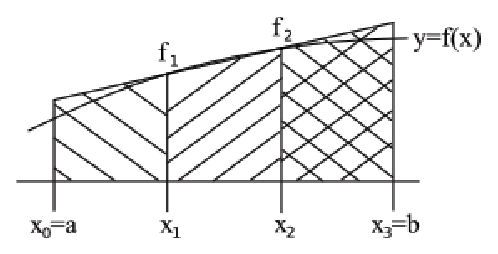
\includegraphics[scale=1.0]{capitulos/capitulo2/figuras/formula_newton_cotes1.eps}
 \caption{Exemplo para $N = 1$ (trapézio)}
 \label{fig:formula_newton_cotes1}
\end{figure}

\[
 \int_a^b f\,(x) \, dx = \alpha \, h \, \left[ w_0\,f_0 + w_1\,f_1 + \dots + w_{n+2}\,f_{n+2} \right] + E
\]

\begin{table}[htp]
\footnotesize
	\centering
		
		\begin{tabular}{|c|c|c|c|}
		\hline		
		\textbf{N} & \textbf{$\alpha$} & \textbf{$w_i\,,\,i=0\,,\,\ldots\,,\,N+2$} & \textbf{E} \\
		\hline \hline
		1 & 3/2 & 0 1 1 0 & $- \displaystyle \frac{1}{4} \, h^3 \, f''$ \\
		\hline 
		2 & 4/3 & 0 2 -1 2 0 & $- \displaystyle \frac{28}{90} \, h^5 \, f^{(iv)}$ \\
		\hline 
		3 & 5/24 & 0 11 1 1 11 0 & $- \displaystyle \frac{95}{144} \, h^5 \, f^{(iv)}$ \\
		\hline 
		4 & 6/20 & 0 11 -14 26 -14 11 0 & $- \displaystyle \frac{41}{140} \, h^7 \, f^{(vi)}$ \\
		\hline 
		\end{tabular}
	\caption{Fórmulas abertas de Newton-Cotes.}
	\label{cap2:sec5:tab1}
\end{table}

\end{enumerate}

\begin{example}

\esp{N = 1}

\begin{figure}[htb]
 \centering
 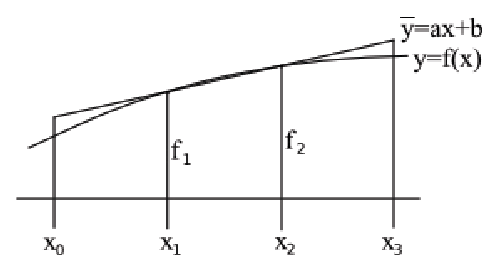
\includegraphics[scale=1.0]{capitulos/capitulo2/figuras/formula_newton_cotes2.eps}
 \caption{Outro exemplo para $N = 1$ (trapézio)}
 \label{fig:formula_newton_cotes2}
\end{figure}

\[
 \begin{array}{ll}
  I = \mbox{ área do trapézio } & = \displaystyle \frac{1}{2} \, (f_0 + f_3) \, 3\,h = \frac{1}{2} \, (f_1 + f_2) \, 3\,h \\ \\
                                & = \displaystyle \frac{3}{2} \, h \, [0 \, f_0 + 1 \, f_1 + 1 \, f_2 + 0 \, f_3]
 \end{array}
\]

\[
 N = 2 \rightarrow g\,(x_1 + s\,h) = f_1 + (f_2 - f_1) \, s + \frac{1}{2} \, (f_3 - 2\,f_2 + f_1)\,(s^2 - s)
\]

\[
\begin{array}{l}
 \begin{array}{l}
  x = x_1 + h\,s \\
  x = x_0 \rightarrow s = -1 \\
  x = x_4 \rightarrow s = 3
 \end{array}
 \qquad
 \begin{array}{ll}
  \displaystyle \int_{x_0}^{x_4} g\,(x) \, dx & = \displaystyle \int_{-1}^3 g\,(x_1 + s\,h) \, h\,ds \\
                                & = \displaystyle \frac{4}{3} \, h \left\{ 0\,f_0 + 2\,f_1 - 1\,f_2 + 2\,f_3 + 0\,f_4 \right\}
 \end{array}
\end{array}
\]

\end{example}

\begin{example}
 Deducão de fórmula de newton-cotes de grau 4.

Temos que:

\emph{\[
I=\int_{a}^{b}{\scriptstyle f(x)dx}=\int_{a}^{b}{\scriptstyle g(x)dx}+E\]
}

De acordo com a regra de interpolacão de Newton 2.4.6 (pág 37 do livro
Applied Numerical methods in C, Nakamura), temos que a formula que
passar pelos K+1 pontos amostrais, $f_{0},f_{1},f_{2}...f_{k}$é dada
pela fórmula:

\[
g({\scriptstyle x})=g({\scriptstyle x_{0}+sh})=\sum_{n=0}^{k}{\scriptstyle \left(_{n}^{s}\right)\triangle^{n}f_{0}}\]


Então, podemos dizer que x está em funcão de s da seguinte forma:

\[
x\left(s\right)=x_{0}+sh\]


\[
dx=h.ds\]


Substituindo e aplicando n=4, temos:

\[
I=\int_{a}^{b}{\scriptstyle g(x)dx}=\int_{0}^{4}{\scriptstyle g(x(s))h.ds}=h\int_{0}^{4}{\scriptstyle g(x_{0}+sh)ds}\]


Sendo que:

\[
g(x)=g(x_{0}+sh)=\sum_{n=0}^{k}{\scriptstyle \left(_{n}^{s}\right)\triangle^{n}f_{0}}\]


Então desenvolvendo o somatório acima, teremos:

\[
g(x_{0}+sh)=g_{0}+s(g_{1}-g_{0})+\frac{s(s-1)}{2}(g{}_{2}-g{}_{1}+g_{0})+\frac{s^{3}-3s^{2}+2s}{6}(g_{3}-3g_{2}+3g_{1}-g_{0})\]


\[
+\frac{s(s-1)(s-2)(s-3)}{24}(g_{4}-4g_{3}+6g_{2}-4g_{1}+g_{0})\]


Substituindo na integral:

\[
h\int_{0}^{4}{\scriptstyle g_{0}+s(g_{1}-g_{0})+\frac{s(s-1)}{2}(g{}_{2}-g{}_{1}+g_{0})+\frac{s^{3}-3s^{2}+2s}{6}(g_{3}-3g_{2}+3g_{1}-g_{0})+\frac{s(s-1)(s-2)(s-3)}{24}(g_{4}-4g_{3}+6g_{2}-4g_{1}+g_{0})}\]


Integrando e isolando por$g_{k}$, temos:

\[
I\equiv h(\frac{14}{45}g_{0}+\frac{64}{45}g_{1}+\frac{24}{45}g_{2}+\frac{64}{45}g_{3}+\frac{14}{45}g_{4})\]


\[
I\equiv\frac{2h}{45}(7g_{0}+32g_{1}+12g_{2}+32g_{3}+7g_{4})_{\blacksquare}\]
\end{example}

